

\section{Actividad 3}

\paragraph{Crear una actividad lúdica para introducir el lenguaje algebraico}

Esto es una actividad para el primer día de clase. La clase tendrá 2 partes.

\subsection{Primera parte}


La primera parte les expondremos un juego de \textit{Matemagia}.
%
En el juego nos presentaremos como un mago, capaz de adivinar un número que hayan pensado.
%
Les diremos "piensa un número" y a continuación una serie de operaciones matemáticas: multiplícalo por 4, súmale 3, restale 5, divídelo por 2...
%
Al final les pediremos el resultado y seremos capaces de adivinar el número que habían pensado inicialmente.
%
En realidad, no es más que despejar una ecuación de primer grado sencilla, que es algo que a final del tema deberían ser capaces de hacer todos.



\paragraph{Ejemplo:}

Piensa un número. Multiplícalo por 2 y súmale 5. ¿Qué resultado has obtenido?

Si pensaron en el 3: $ 3\to 2·3 = 6\to 6+5 = 11 $, con lo que nuestra labor sería, dado el resultado $11$ y siendo $x$ el número que inicialmente han pensado:

\[
	2x+5 = 11 \to x = \frac{11-5}{2} = 3
\]

Sabiendo el resultado final, somos capaces de adivinar el número inicial.

\paragraph{Ejemplo 2:}(algo más complicado)

Piensa un número. Súmale 3, multiplícalo por 2, réstale 7. ¿Qué resultado has obtenido?

\[
(x + 3)·2 - 7 = y \to x = \frac{y+7}{2} - 3
\]


Cada ejemplo se puede utilizar varias veces, de hecho, incluso puede usarse siempre el mismo.

\textit{El objetivo de este juego es hacerles interesante el álgebra y despertarles  ganas de aprender.
%
Les diremos que no les vamos a desvelar el secreto hasta dentro de 1 mes, cuando hayamos acabado el tema.
%
Entonces, ellos serán capaces de plantear este tipo de acertijos.
%
Este juego además, nos puede permitir, si durante el tema han perdido la ilusión por el álgebra, recordarles lo chulo que será cuando sepan crear este tipo de acertijos y que deberían esforzarse por aprender, aunque sea para vacilar a sus padres con este truquillo de matemagia.
}

\newpage

\subsection{Segunda parte}

La segunda les presentamos un acertijo a resolver por grupos de 4. Cada grupo recibirá una cartulina con la siguiente imagen:

\begin{center}
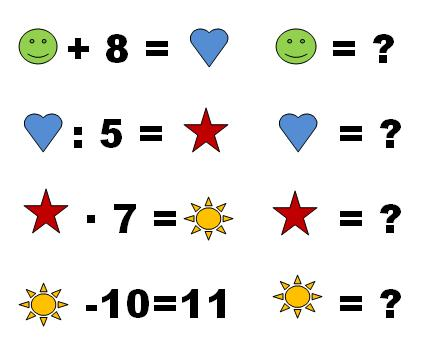
\includegraphics[scale=0.8]{../../img/introAlgebra.jpg}
\end{center}

Cada símbolo representa un número, y el objetivo es resolver cuánto vale cada símbolo y que de esta manera se familiaricen con la idea "un símbolo representa un número".
%
Aunque todavía no lo han visto, viendo la última ecuación, alguno del grupo se dará cuenta que el sol debería ser un 21 para que eso fuera una igualdad. Con el sol, de abajo arriba podrán resolver las demás ecuaciones.


Una vez resuelto el acertijo, se les entregará (si da tiempo) un acertijo similar, pero cada incógnita estará representada por una letra en vez de por un símbolo.


De esta manera ellos habrán participado muy activamente en su proceso de aprendizaje de que los símbolos pueden representar números, que es la base del lenguaje algebraico.

